\documentclass[12pt,a4paper]{article}
\usepackage[utf8]{inputenc} % inutile avec XeLaTeX/LuaLaTeX
\usepackage[T1]{fontenc}
\usepackage{amsmath,amssymb,mathrsfs,tikz,times,pifont}
\usepackage{enumitem}
\usepackage{multicol}
\usepackage{lmodern}
\newcommand\circitem[1]{%
\tikz[baseline=(char.base)]{
\node[circle,draw=gray, fill=red!55,
minimum size=1.2em,inner sep=0] (char) {#1};}}
\newcommand\boxitem[1]{%
\tikz[baseline=(char.base)]{
\node[fill=cyan,
minimum size=1.2em,inner sep=0] (char) {#1};}}
\setlist[enumerate,1]{label=\protect\circitem{\arabic*}}
\setlist[enumerate,2]{label=\protect\boxitem{\alph*}}
\everymath{\displaystyle}
\usepackage[left=1cm,right=1cm,top=1cm,bottom=1.7cm]{geometry}
\usepackage[colorlinks=true, linkcolor=blue, urlcolor=blue, citecolor=blue]{hyperref}
\usepackage{array,multirow}
\usepackage[most]{tcolorbox}
\usepackage{varwidth}
\usepackage{float}
\tcbuselibrary{skins,hooks}
\usetikzlibrary{patterns}

\newtcolorbox{exa}[2][]{enhanced,breakable,before skip=2mm,after skip=5mm,
colback=yellow!20!white,colframe=black!20!blue,boxrule=0.5mm,
attach boxed title to top left ={xshift=0.6cm,yshift*=1mm-\tcboxedtitleheight},
fonttitle=\bfseries,
title={#2},#1,
boxed title style={frame code={
\path[fill=tcbcolback!30!black]
([yshift=-1mm,xshift=-1mm]frame.north west)
arc[start angle=0,end angle=180,radius=1mm]
([yshift=-1mm,xshift=1mm]frame.north east)
arc[start angle=180,end angle=0,radius=1mm];
\path[left color=tcbcolback!60!black,right color = tcbcolback!60!black,
middle color = tcbcolback!80!black]
([xshift=-2mm]frame.north west) -- ([xshift=2mm]frame.north east)
[rounded corners=1mm]-- ([xshift=1mm,yshift=-1mm]frame.north east)
-- (frame.south east) -- (frame.south west)
-- ([xshift=-1mm,yshift=-1mm]frame.north west)
[sharp corners]-- cycle;
},interior engine=empty,
},interior style={top color=yellow!5}}

\usepackage{fancyhdr}
\usepackage{eso-pic}
\usepackage{tkz-tab}
\AddToShipoutPicture{
    \AtTextCenter{%
        \makebox[0pt]{\rotatebox{80}{\textcolor[gray]{0.7}{\fontsize{5cm}{5cm}\selectfont PGB}}}
    }
}

\usepackage{verbatim}

\usepackage{color,soul}

\usepackage{amsmath}
\usepackage{amsfonts}
\usepackage{amssymb}
\usepackage{systeme}
\usepackage{tkz-tab}
\usepackage{tikz}
\usepackage{enumitem}
\usepackage{tcolorbox}
\usepackage{lmodern}
\usepackage{geometry}
\usepackage{multirow}
\usepackage{diagbox}
\usepackage{pgfplots}
\usetikzlibrary{arrows}
\newcounter{exemple} % Compteur pour les questions

% Définir la commande pour afficher une question numérotée
\newcommand{\exemple}{%
  \refstepcounter{exemple}%
  \textbf{\textcolor{green}{Exemple \theexemple :}} \ignorespaces
}
%---------------------------------------
\definecolor{myorange}{rgb}{1.0, 0.8, 0.0}

% Définir un compteur pour les exercices d'application
\newcounter{exerciceapp}

% Définir la commande pour afficher un exercice d'application numéroté
\newcommand{\exerciceapp}{%
  \refstepcounter{exerciceapp}%
  \textbf{\textcolor{myorange}{Exercice d'application \theexerciceapp :}} \ignorespaces
}
%--------------------------------------
% Définir un compteur pour les exercices d'application
\newcounter{correction}

% Définir la commande pour afficher un correction exercice d'application numéroté
\newcommand{\correction}{%
  \refstepcounter{correction}%
  \textbf{\textcolor{myorange}{Correction \thecorrection :}} \ignorespaces
}
%--------------------------------------
% Commande pour ajouter du texte en arrière-plan
\usepackage{fancyhdr}
\usepackage{eso-pic}
%\usepackage{tkz-tab}
\AddToShipoutPicture{
    \AtTextCenter{%
        \makebox[0pt]{\rotatebox{80}{\textcolor[gray]{0.7}{\fontsize{5cm}{5cm}\selectfont PGB}}}
    }
}
%This command takes a colour as an optional argument; the default colour is black.
\usetikzlibrary{shapes.geometric,fit}
\newcommand{\myul}[2][black]{\setulcolor{#1}\ul{#2}\setulcolor{black}}
\newcommand\tab[1][1cm]{\hspace*{#1}}

\begin{document}
% En-tête personnalisée
\begin{center}
    \Large\fcolorbox{green}{white}{\textbf{\textcolor{red}{CHAP 10 : LES STATISTIQUES}}}\\[-0.1cm]
    \normalsize\textbf{Prof : M. BA} \hfill \textbf{Classe : TS2}\\[-0.1cm]
    \textbf{Année scolaire : 2024 -- 2025}
\end{center}

\section*{\textcolor{red}{I. \underline{VOCABULAIRE}}}

\begin{enumerate}
    \item \textbf{\underline{Population}} : C’est l’ensemble des individus sur les quels porte une étude statistique.
    \item \textbf{\underline{Échantillon}} : C’est une partie de la population.
    \item \textbf{\underline{Caractère}} : Le caractère est l’information sur laquelle l’étude statistique est réalisée. Il peut être quantitatif s’il est mesurable, exemple \textit{la taille, la masse}, etc., ou qualitatif dans le cas contraire, exemple \textit{la couleur, la nationalité}, etc.
    \item \textbf{\underline{Effectif}} : C’est le nombre d’individus d’une population ou d’une partie de cette population.
    \item \textbf{\underline{Modalité}} : C’est l’une des différentes valeurs ou qualités de la variable d’une série statistique.
    \item \textbf{\underline{Fréquence}} : C’est le nombre de fois qu’une modalité est représentée par rapport à l’effectif total. Elle est donc toujours inférieure à 1 et la somme totale de toutes les fréquences donne 1.
\end{enumerate}

\section*{\textcolor{red}{Exemple illustratif du vocabulaire statistique}}

\begin{tcolorbox}[colback=gray!5, colframe=black, title=\textbf{Situation}]
Un professeur interroge les élèves d’une classe de 4\textsuperscript{e} (soit 25 élèves) pour connaître leur moyen de transport principal pour venir à l’école. Il note les réponses suivantes :
\begin{center}
\textit{Bus, Bus, Voiture, Marche, Bus, Vélo, Voiture, Bus, Vélo, Bus, Voiture, Bus, Marche, Vélo, Bus, Bus, Bus, Voiture, Marche, Bus, Vélo, Voiture, Bus, Vélo, Bus}
\end{center}
\end{tcolorbox}

\vspace{0.5cm}

\textbf{Analyse :}
\begin{itemize}
    \item \textbf{Population} : L’ensemble des 25 élèves de la classe.
    \item \textbf{Individu} : Chaque élève interrogé.
    \item \textbf{Échantillon} : Si on avait choisi uniquement 10 élèves sur les 25, cela aurait constitué un échantillon.
    \item \textbf{Caractère} : Le moyen de transport utilisé pour venir à l’école. C’est un caractère \textbf{qualitatif}.
    \item \textbf{Modalités} : Les différentes réponses possibles : \textit{Bus, Voiture, Marche, Vélo}.
    \item \textbf{Effectifs} :
    \begin{itemize}
        \item Bus : 12 élèves
        \item Voiture : 5 élèves
        \item Marche : 3 élèves
        \item Vélo : 5 élèves
    \end{itemize}
    \item \textbf{Fréquences} :
    \begin{itemize}
        \item Bus : \( \frac{12}{25} = 0{,}48 \)
        \item Voiture : \( \frac{5}{25} = 0{,}20 \)
        \item Marche : \( \frac{3}{25} = 0{,}12 \)
        \item Vélo : \( \frac{5}{25} = 0{,}20 \)
    \end{itemize}
\end{itemize}

\section*{\textcolor{red}{II. \underline{SÉRIE STATISTIQUE D’UNE VARIABLE}}}

\subsection*{\textcolor{red}{1. Définition}}

On appelle série statistique d’une variable \( x \) ou série statistique simple, la série obtenue si l’étude est réalisée sur un seul caractère \( x \). Elle peut être \textit{groupée} ou \textit{non groupée} en classes.\\
On la note \( (x_i, n_i) \). Avec \( x = \{x_1, x_2, \dots, x_p\} \) et \( n_i \) est l’effectif de la modalité \( x_i \).

\subsection*{\textcolor{red}{2. \underline{Effectif total, Moyenne, Variance, Écart-type, Fréquence partielle, Espérance}}}

\textbf{\textit{Effectif total}} : 
\fcolorbox{red}{red!20}{$N = \sum\limits_{i=1}^{p} n_i$} \quad 
\textbf{Moyenne} : 
\fcolorbox{red}{red!20}{$\bar{x} = \frac{1}{N} \sum\limits_{i=1}^{p} n_i x_i$}

\vspace{0.2cm}

Si la série est \textit{groupée en classes}, alors : 
\noindent
\fcolorbox{red}{red!20}{
\(\bar{x} = \frac{1}{N} \sum\limits_{i=1}^{p} n_i c_i\)
}
\quad où \(c_i = \frac{a + b}{2}\), le centre de la classe \(i\) de la forme \([a~;~b[\).

\vspace{0.2cm}

\textbf{Variance} : 
\fcolorbox{red}{red!20}{$V(x) = \frac{1}{N} \sum\limits_{i=1}^{p} n_i x_i^2 - \bar{x}^2$}

\vspace{0.2cm}

Si la série est groupée en classes alors :

\textbf{Variance} : 
\fcolorbox{red}{red!20}{$V(x) = \frac{1}{N} \sum\limits_{i=1}^{p} n_i c_i^2 - \bar{x}^2$} \quad \textit{La variance est toujours positive.}

\vspace{0.2cm}

\textbf{Écart-type} : 
\fcolorbox{red}{red!20}{$\sigma(x) = \sqrt{V(x)}$} \quad 
\textbf{Fréquence partielle} : 
\fcolorbox{red}{red!20}{$f_i = \dfrac{n_i}{N}$}

\[
\fcolorbox{red}{red!20}{$\sum\limits_{i=1}^{p} f_i = 1$}
\]

\noindent
\textbf{\textcolor{red}{Exemple}} : On représente au tableau N\textsuperscript{o}1 les tailles en cm de 10 jeunes garçons et au tableau N\textsuperscript{o}2, les notes en maths de 11 élèves d’une classe de TS2.

\vspace{0.5cm}

\begin{center}
\textbf{Tableau N\textsuperscript{o}1}

\vspace{0.2cm}
\begin{tabular}{|c|c|c|c|c|c|}
\hline
Tailles \( x_i \) en cm & 170 & 172 & 175 & 180 & 185 \\
\hline
Effectifs \( n_i \) & 1 & 2 & 3 & 3 & 1 \\
\hline
\end{tabular}
\end{center}

\vspace{1cm}

\begin{center}
\textbf{Tableau N\textsuperscript{o}2}

\vspace{0.2cm}
\begin{tabular}{|c|c|c|c|c|c|}
\hline
Notes en maths \( x_i \) & [8;10[ & [10;12[ & [12;14[ & [14;16[ & [16;18[ \\
\hline
Effectifs \( n_i \) & 3 & 4 & 2 & 1 & 1 \\
\hline
\end{tabular}
\end{center}

\vspace{0.5cm}

\noindent
Pour chacun des tableaux ci-dessus, déterminer l’effectif total, la moyenne, la variance, l’écart-type et les fréquences partielles.

\noindent
\textbf{\textcolor{red}{Solution}}

\begin{itemize}
    \item \textbf{Tableau N\textsuperscript{o}1 :} Série non groupée en classes.\\
    \( N = 1 + 2 + 3 + 3 + 1 = 10. \)\\[0.2cm]
    \( 
    \bar{x} = \frac{1}{10} (1 \times 170 + 2 \times 172 + 3 \times 175 + 3 \times 180 + 1 \times 185) = 176{,}4~\text{cm}.
    \)\\[0.2cm]
    \( 
    V(x) = \frac{1}{10} (1 \times 170^2 + 2 \times 172^2 + 3 \times 175^2 + 3 \times 180^2 + 1 \times 185^2) - (176{,}4)^2 = 19{,}84.
    \)\\[0.2cm]
    \( 
    \sigma(x) = \sqrt{19{,}84} = 4{,}45.
    \)\\[0.2cm]
    \( 
    f_1 = \frac{1}{10} \quad ; \quad 
    f_2 = \frac{2}{10} \quad ; \quad 
    f_3 = \frac{3}{10} \quad ; \quad 
    f_4 = \frac{3}{10} \quad \text{et} \quad 
    f_5 = \frac{1}{10}.
    \)

    \vspace{0.5cm}
    
    \item \textbf{Tableau N\textsuperscript{o}2 :} Série groupée en classes.\\
    \( N = 3 + 4 + 2 + 1 + 1 = 11. \)\\[0.2cm]
    \[
    \bar{x} = \frac{1}{11} \left[ 
    3 \times \left( \frac{8 + 10}{2} \right)
    + 4 \times \left( \frac{10 + 12}{2} \right)
    + 2 \times \left( \frac{12 + 14}{2} \right)
    + 1 \times \left( \frac{14 + 16}{2} \right)
    + 1 \times \left( \frac{16 + 18}{2} \right)
    \right] = 11{,}73.
    \]\\[0.2cm]
    \[
    V(x) = \frac{1}{11} \left( 
    3 \times 9^2 + 4 \times 11^2 + 2 \times 13^2 + 1 \times 15^2 + 1 \times 17^2 
    \right) - (11{,}73)^2 = 5{,}95.
    \]\\[0.2cm]
    \( 
    \sigma(x) = \sqrt{5{,}95} = 2{,}44.
    \)\\[0.2cm]
    \( 
    f_1 = \frac{3}{11} \quad ; \quad 
    f_2 = \frac{4}{11} \quad ; \quad 
    f_3 = \frac{2}{11} \quad ; \quad 
    f_4 = \frac{1}{11} \quad \text{et} \quad 
    f_5 = \frac{1}{11}.
    \)
\end{itemize}

\section*{\textcolor{red}{III. \underline{SÉRIE STATISTIQUE DE DEUX VARIABLES}}}

\subsection*{\textcolor{red}{1. \underline{Définitions : Cas général, série non injective}}}

On appelle série statistique de deux variables \( x \) et \( y \), ou série statistique double, la série obtenue si l’étude est réalisée à la fois sur deux caractères différents \( x \) et \( y \). \\
Elle est donc formée de deux séries simples qui peuvent être groupées ou non ; ou l’une peut être groupée et l’autre non groupée.\\
On la note \( (x_i, y_j, n_{ij}) \). On la représente dans un tableau à double entrée appelé tableau de contingence.

\vspace{0.2cm}
Si \( x = \{x_1, x_2, \dots, x_p\} \) et \( y = \{y_1, y_2, \dots, y_q\} \), alors :

\begin{itemize}
    \item \( n_{ij} \) est l’effectif du couple \( (x_i, y_j) \). L’effectif total sera 
    \fcolorbox{red}{red!20}{$N = \sum\limits_{i=1}^{p} \sum\limits_{j=1}^{q} n_{ij}$}
    \item 
    \fcolorbox{red}{red!20}{$
    n_{i\bullet} = n_{i1} + n_{i2} + \cdots + n_{iq} \quad \text{et} \quad 
    n_{\bullet j} = n_{1j} + n_{2j} + \cdots + n_{pj}$
    }
    sont respectivement les effectifs partiels sur la ligne \( i \) et sur la colonne \( j \).
    
    \item 
    \fcolorbox{red}{red!10}{$
    f_{ij} = \frac{n_{ij}}{N}$}
    $\quad \text{est la fréquence du couple } (x_i, y_j). \quad $
    \fcolorbox{red}{red!10}{$
    f_{i\bullet} = \frac{n_{i\bullet}}{N} \quad \text{et} \quad f_{\bullet j} = \frac{n_{\bullet j}}{N}$
    }sont les fréquences partielles sur la ligne $i$ et la colonne $j$.

    \item Les fréquences conditionnelles : 
    \fcolorbox{red}{red!20}{$
    f_{x_i/y_j} = \frac{n_{ij}}{n_{\bullet j}} \quad \text{et} \quad 
    f_{y_j/x_i} = \frac{n_{ij}}{n_{i\bullet}}$
    }

    \item On appelle \textbf{nuage de points} l’ensemble des points \( M(x_i ; y_j) \), que l’on notera \( M_{ij} \) dans un repère.\\
    On appelle \textbf{point moyen} le point \( G \), barycentre des points \( (M_{ij} ; n_{ij}) \).

    \item On appelle \textbf{covariance} d’une série statistique de deux variables \( x \) et \( y \), le réel noté :

    \fcolorbox{red}{red!20}{$
    \textbf{Cov}(x, y) = \frac{1}{N} \sum\limits_{i=1}^{p} \sum\limits_{j=1}^{q} n_{ij} x_i y_j - \bar{x} \cdot \bar{y}$
    }

\end{itemize}
\noindent
\textbf{\textcolor{red}{\underline{Exemple}}} : Le tableau ci-dessous représente les notes \( x \) en Maths et les notes \( y \) en PC de 10 élèves d’une classe de TS\textsubscript{2}.

\vspace{0.5cm}

\begin{center}
\begin{tabular}{|c|c|c|c|}
\hline
\diagbox[width=6em, height=3em]{$x_i$}{$y_j$} & \textbf{8} & \textbf{11} & \textbf{12} \\
\hline
\textbf{9} & 2 & 0 & 0 \\
\hline
\textbf{10} & 0 & 3 & 1 \\
\hline
\textbf{11} & 0 & 1 & 2 \\
\hline
\textbf{12} & 0 & 0 & 1 \\
\hline
\end{tabular}
\end{center}
\begin{enumerate}
    \item Donner la valeur de \( n_{23} \). Interpréter cette valeur.
    \item Déterminer les séries marginales de \( x \) et \( y \), puis donner \( \bar{x} \) et \( \bar{y} \).
    \item Déterminer la série conditionnelle \( z = x \,/\,_{y=12} \). Calculer sa moyenne puis l’interpréter.
    \item Déterminer \( f_{3\bullet} \) et \( f_{\bullet2} \).
    \item Calculer \( \text{cov}(x, y) \).
\end{enumerate}

\noindent \textbf{\textcolor{red}{Solution}}

\begin{enumerate}
    \item \( n_{23} \) est la valeur qui se situe sur la deuxième ligne et la troisième colonne.\\
    Donc \( n_{23} = 1 \). Ça veut dire qu’il y a 1 seul élève qui a 10 en Maths et 12 en PC.
    
    \item La série marginale de \( x \) : (On extrait la série de \( x \) de la série double)

    \begin{center}
    \begin{tabular}{|c|c|c|c|c|}
    \hline
    Notes de Maths \( x_i \) & 9 & 10 & 11 & 12 \\
    \hline
    Effectifs \( n_i \) & 2 & 4 & 3 & 1 \\
    \hline
    \end{tabular}
    \end{center}

    \[
    \bar{x} = \frac{1}{10}(2 \times 9 + 4 \times 10 + 3 \times 11 + 1 \times 12) = 10{,}3
    \]

    La série marginale de \( y \) : (On extrait la série de \( y \) de la série double)

    \begin{center}
    \begin{tabular}{|c|c|c|c|}
    \hline
    Notes de PC \( y_j \) & 8 & 11 & 12 \\
    \hline
    Effectifs \( n_j \) & 2 & 4 & 4 \\
    \hline
    \end{tabular}
    \end{center}

    \[
    \bar{y} = \frac{1}{10}(2 \times 8 + 4 \times 11 + 4 \times 12) = 10{,}8
    \]
\end{enumerate}
\begin{enumerate}
    \setcounter{enumi}{2} % pour commencer à la question 3
    \item La série conditionnelle \( z = x \,/\,_{y=12} \) :

    \begin{center}
    \begin{tabular}{|c|c|c|c|}
    \hline
    \( z_i = x_i /_{y=12} \) & 10 & 11 & 12 \\
    \hline
    \( n_i \) & 1 & 2 & 1 \\
    \hline
    \end{tabular}
    \end{center}

    \[
    \bar{z} = \frac{1}{4}(1 \times 10 + 2 \times 11 + 1 \times 12) = 11.
    \]
    C’est la moyenne en Maths des élèves qui ont 12 en PC.

    \item Déterminer \( f_{3.} \) et \( f_{.2} \).

    \[
    f_{3.} = \frac{n_{3.}}{10} \quad \text{et } n_{3.} = 0 + 1 + 2 = 3 \quad \Rightarrow \quad f_{3.} = \frac{3}{10}
    \]
    \[
    f_{.2} = \frac{n_{.2}}{10} \quad \text{et } n_{.2} = 0 + 3 + 1 + 0 = 4 \quad \Rightarrow \quad f_{.2} = \frac{4}{10}
    \]

    \item La covariance de \( x \) et \( y \).

    \(
    \text{Cov}(x, y) = \frac{
    (2 \times 8 \times 9 + 3 \times 11 \times 10 + 1 \times 12 \times 10 + 1 \times 11 \times 11 + 2 \times 12 \times 11 + 1 \times 12 \times 12)
    }{10} - 10{,}3 \times 10{,}8 = 1{,}06.
    \)
\end{enumerate}

\subsection*{\textcolor{red}{2. Cas particulier : Série injective}}

Une série est dite injective si : 
\fcolorbox{red}{red!10}{$n_{ij} = 
\begin{cases}
1 & \text{si } i = j \\
0 & \text{si } i \ne j
\end{cases}$}. 
Elle est notée 
\fcolorbox{red}{red!10}{$(x_i ; y_i)$} 
et se présente sous forme d’un tableau de deux lignes de même longueur.\\
Dans ce cas, l’effectif total \( N \) est le nombre de couples \( (x_i ; y_i) \).

\vspace{0.3cm}

\begin{itemize}
    \item 
    \fcolorbox{red}{red!10}{$\bar{x} = \frac{1}{N} \sum\limits_{i=1}^{p} x_i$} 
    \quad et \quad 
    \fcolorbox{red}{red!10}{$\bar{y} = \frac{1}{N} \sum\limits_{i=1}^{p} y_i$}
    \quad si la série n’est pas groupée en classes.

    \item 
    \fcolorbox{red}{red!10}{$\bar{x} = \frac{1}{N} \sum\limits_{i=1}^{p} n_i c_i$}
    \quad et \quad 
    \fcolorbox{red}{red!10}{$\bar{y} = \frac{1}{N} \sum\limits_{i=1}^{p} n_i c_i$}
    \quad si la série est groupée en classes.

    \item 
    \fcolorbox{red}{red!10}{$V(x) = \frac{1}{N} \sum\limits_{i=1}^{p} x_i^2 - \bar{x}^2$} 
    \quad et \quad 
    \fcolorbox{red}{red!10}{$V(y) = \frac{1}{N} \sum\limits_{i=1}^{p} y_i^2 - \bar{y}^2$}

     Plus simplement on a :
    \fcolorbox{red}{red!10}{$V(x) = \overline{x^2} - \bar{x}^2$} 
    \quad et \quad 
    \fcolorbox{red}{red!10}{$V(y) = \overline{y^2} - \bar{y}^2$}

    \item 
    \fcolorbox{red}{red!10}{$\sigma(x) = \sqrt{V(x)}$}
    \quad et \quad 
    \fcolorbox{red}{red!10}{$\sigma(y) = \sqrt{V(y)}$}

    \item 
    \fcolorbox{red}{red!10}{$\text{Cov}(x, y) = \frac{1}{N} \sum\limits_{i=1}^{p} x_i y_i - \bar{x} \bar{y}$}
    \quad ou plus simplement :
    \fcolorbox{red}{red!10}{$\text{Cov}(x, y) = \overline{xy} - \bar{x} \cdot \bar{y}$}
\end{itemize}

\vspace{0.3cm}
Le \textit{nuage de points} est l’ensemble des points \( M(x_i ; y_i) \) dans un repère.\\
Le \textbf{point moyen} est le point 
\fcolorbox{red}{red!10}{$G(\bar{x} ; \bar{y})$}, 
il sera toujours au centre du nuage (Isobarycentre).

\noindent
\subsection*{\textcolor{red}{Exemple : Série non groupée en classes}} : On donne le tableau statistique ci-dessous :

\vspace{0.5cm}

\begin{center}
\begin{tabular}{|c|c|c|c|c|}
\hline
\( x_i \) & 2 & 4 & 5 & 7 \\
\hline
\( y_i \) & 1 & 2 & 3 & 4 \\
\hline
\end{tabular}
\end{center}

\vspace{0.5cm}

\begin{enumerate}
    \item Représenter le nuage de points de cette série statistique.
    \item Calculer \( \bar{x}, \bar{y}, V(x), V(y) \) et \( \text{Cov}(x, y) \).
    \item Représenter le point moyen \( G \) dans le nuage.
\end{enumerate}
\noindent \textbf{\textcolor{red}{Solution}}

\begin{enumerate}
    \item Le nuage de points
\begin{center}
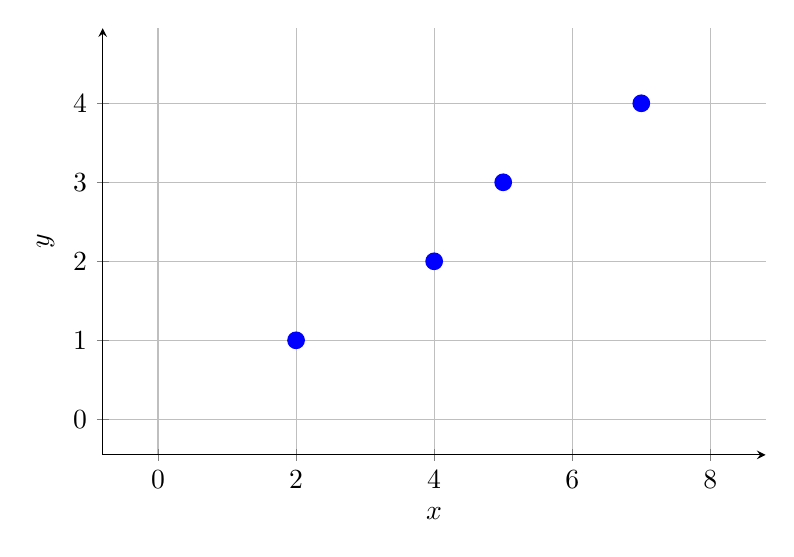
\begin{tikzpicture}
\begin{axis}[
    axis lines = left,
    xlabel = {$x$},
    ylabel = {$y$},
    xmin=0, xmax=8,
    ymin=0, ymax=4.5,
    xtick={0,2,4,6,8},
    ytick={0,1,2,3,4},
    grid = both,
    width=10cm,
    height=7cm,
    enlargelimits
]
\addplot[
    only marks,
    mark=*,
    mark size=3pt,
    blue
]
coordinates {
    (2,1)
    (4,2)
    (5,3)
    (7,4)
};
\end{axis}
\end{tikzpicture}
\end{center}

\begin{itemize}
    \item Si le nuage de points a la forme d’une droite, alors les variables \( x \) et \( y \) sont liées par une relation linéaire qu’on verra plus tard dans la suite du cours.
\end{itemize}
    \item \hspace{1cm}
    \begin{center}
    \begin{tabular}{|c|c|c|c|c|c|}
    \hline
      &  &  &  &  & \textbf{Total} \\
    \hline
    \( x_i \) & 2 & 4 & 5 & 7 & 18 \\
    \hline
    \( y_i \) & 1 & 2 & 3 & 4 & \textbf{10} \\
    \hline
    \( x_i^2 \) & 4 & 16 & 25 & 49 & \textbf{94} \\
    \hline
    \( y_i^2 \) & 1 & 4 & 9 & 16 & \textbf{30} \\
    \hline
    \( x_i y_i \) & 2 & 8 & 15 & 28 & \textbf{53} \\
    \hline
    \end{tabular}
    \end{center}

    \[
    \bar{x} = \frac{18}{4} = 4{,}5 \quad ; \quad
    \bar{y} = \frac{10}{4} = 2{,}5
    \quad ; \quad
    V(x) = \frac{94}{4} - (4{,}5)^2 = 3{,}25
    \quad ; \quad
    V(y) = \frac{30}{4} - (2{,}5)^2 = 1{,}25
    \]

    \[
    \text{Cov}(x, y) = \frac{53}{4} - 4{,}5 \times 2{,}5 = 2
    \]

    \item Le point moyen est donc \( G(4{,}5 \, ; \, 2{,}5) \). On peut le placer dans le nuage.
\end{enumerate}
\subsection*{\textcolor{red}{Exemple : Série groupée en classes}}

\textbf{Durées de connexion (en minutes) de 40 élèves sur une plateforme :}

\begin{center}
\begin{tabular}{|c|c|c|c|c|c|}
\hline
Classe & [0 ; 10[ & [10 ; 20[ & [20 ; 30[ & [30 ; 40[ & [40 ; 50[ \\
\hline
Effectif \( n_i \) & 5 & 8 & 12 & 10 & 5 \\
\hline
Centre \( c_i \) & 5 & 15 & 25 & 35 & 45 \\
\hline
\end{tabular}
\end{center}

\vspace{0.5cm}

Effectif total : \( N = 5 + 8 + 12 + 10 + 5 = 40 \)

\(\begin{aligned}
    \bar{x} &= \frac{1}{40}(5 \times 5 + 8 \times 15 + 12 \times 25 + 10 \times 35 + 5 \times 45)\\\
    &= \frac{5\cdot5 + 8\cdot15 + 12\cdot25 + 10\cdot35 + 5\cdot45}{40}\\
    &= 25
\end{aligned}\)

\(\begin{aligned}
    V(x) &= \frac{1}{40}(5 \cdot 5^2 + 8 \cdot 15^2 + 12 \cdot 25^2 + 10 \cdot 35^2 + 5 \cdot 45^2) - \bar{x}^2\\
&= \frac{5 \cdot 25 + 8 \cdot 225 + 12 \cdot 625 + 10 \cdot 1225 + 5 \cdot 2025}{40} - 625 \\
&= 125
\end{aligned}\)

\[
\sigma(x) = \sqrt{V(x)} = \sqrt{125} \approx 11{,}18
\]

\(\text{Fréquence partielle de la classe } [20 ; 30[ : 
\quad f_3 = \frac{12}{40} = 0{,}3\)

\section*{\textcolor{red}{IV. \underline{AJUSTEMENT LINÉAIRE}}}

\subsection*{\textcolor{red}{1. Coefficient de corrélation}}

On appelle coefficient de corrélation linéaire entre les variables \( x \) et \( y \) (le lien entre les deux variables) d’une série statistique double, le réel


\fcolorbox{red}{red!10}{$
r = \frac{\text{Cov}(x, y)}{\sqrt{V(x) \times V(y)}}$
}
\quad \text{ou encore} \quad
\fcolorbox{red}{red!10}{$
r = \frac{\text{Cov}(x, y)}{\sigma(x) \, \sigma(y)}$
}


\begin{itemize}
    \item On a toujours 
    \fcolorbox{red}{red!10}{\(-1 \leq r \leq 1\)}
    \item Si \( |r| \geq 0{,}87 \) ou \( r^2 \geq 0{,}75 \) alors la \textit{corrélation entre \( x \) et \( y \) est forte}.
    \item Si \( |r| < 0{,}87 \) ou \( r^2 < 0{,}75 \) alors la \textit{corrélation entre \( x \) et \( y \) est faible}.
    \item Si \( r = -1 \) ou \( r = 1 \) alors la \textit{corrélation entre \( x \) et \( y \) est parfaite}.
    \item Si \( r = 0 \), alors la \textit{corrélation entre \( x \) et \( y \) est nulle}.\\
    Dans ce cas, il n’y a aucune relation entre \( x \) et \( y \).\\
    On dira que les variables \( x \) et \( y \) sont \textit{indépendantes}.
\end{itemize}

\vspace{0.2cm}
\noindent
\textbf{\underline{Remarque}} : Quand la corrélation entre deux variables est forte, alors on peut faire une \textbf{estimation} d’une des valeurs connaissant l’autre à l’aide des droites de régression.

\subsection*{\textcolor{red}{2. \underline{Droites de régression : Par la méthode des moindres carrés}}}

On peut déterminer les droites de régression linéaires de la manière ci-dessous, appelée la méthode des moindres carrés :


\fcolorbox{red}{red!10}{$
(D_{y/x}) : y - \bar{y} = a(x - \bar{x}) \quad \text{avec} \quad a = \frac{\text{Cov}(x, y)}{V(x)}$
}
\quad \text{est la droite de régression de \( y \) en \( x \).}



\fcolorbox{red}{red!10}{$
(D_{x/y}) : x - \bar{x} = a'(y - \bar{y}) \quad \text{avec} \quad a' = \frac{\text{Cov}(x, y)}{V(y)}$
}
\quad \text{est la droite de régression de \( x \) en \( y \).}


\begin{itemize}
    \item Après transformation, elles s’écrivent sous la forme : \\
    \( (D_{y/x}) : y = ax + b \quad \text{et} \quad (D_{x/y}) : x = a'y + b' \)
    
    \item On « peut » retrouver \( D_{y/x} \) à partir de \( D_{x/y} \) et réciproquement.

    \item Les droites de régression linéaires passent toujours par le point moyen.

    \item 
    \fcolorbox{red}{red!10}{
    On a toujours \( aa' = r^2 \)
    } \quad (À démontrer).
\end{itemize}
\noindent
\section*{\textcolor{red}{\underline{Exercice d’application}}}

D’après des études scientifiques, la croissance d’un arbre ne s’arrête jamais.\\
On considère un arbre dont la hauteur \( x \) en \textit{mètres} et son âge \( y \) en \textit{années} sont consignés dans le tableau ci-dessous :\\
Les résultats seront donnés à 1 chiffre après la virgule.

\vspace{0.5cm}

\begin{center}
\begin{tabular}{|c|c|c|c|c|}
\hline
\( x_i \) & 3 & 5 & 7{,}5 & 8 \\
\hline
\( y_i \) & 2 & 4 & 6 & 7 \\
\hline
\end{tabular}
\end{center}

\vspace{0.5cm}

\begin{enumerate}
    \item Déterminer le coefficient de corrélation linéaire entre \( x \) et \( y \).
    \item Justifier qu’on peut estimer la hauteur de cet arbre si on connaît son âge.
    \item Quelle serait sa hauteur à l’âge de 10 ans ?
    \item Si l’arbre mesure 11 mètres, estimer son âge en années.
\end{enumerate}
\section*{\textcolor{red}{Correction de l'exercice}}

\begin{enumerate}
    \item \textbf{Détermination du coefficient de corrélation linéaire}

    \[
    r = \frac{\text{Cov}(x, y)}{\sigma(x)\sigma(y)} \approx 0{,}995
    \]

    Il y a donc une \textbf{corrélation linéaire très forte et positive} entre la hauteur et l’âge de l’arbre.

    \item \textbf{Justification de l’utilisation d’une estimation linéaire}

    Comme \( r \approx 1 \), la corrélation est très forte. On peut donc utiliser la droite de régression pour estimer la hauteur de l’arbre à partir de son âge, ou inversement.

    \item \textbf{Estimation de la hauteur à 10 ans}

    Droite de régression de \( y \) en fonction de \( x \) :

    \[
    y = ax + b \quad \text{avec } a \approx 0{,}95 \quad \text{et } b \approx -0{,}83
    \]

    \[
    y(10) = 0{,}95 \times 10 - 0{,}83 = \boxed{8{,}7~\text{mètres}}
    \]

    \item \textbf{Estimation de l’âge si l’arbre mesure 11 mètres}

    Droite de régression de \( x \) en fonction de \( y \) :

    \[
    x = a'y + b' \quad \text{avec } a' \approx 1{,}042 \quad \text{et } b' \approx 0{,}924
    \]

    \[
    y(11) = \frac{11 - 0{,}924}{1{,}042} \approx \boxed{12{,}4~\text{années}}
    \]

\end{enumerate}

\end{document}